\documentclass[ignorenonframetext,xcolor=x11names]{beamer}

\input{../common.preamble.beamer.tex}
 
\title{Business 4720 - Class 4}

\subtitle{Querying Graph and Document Databases}

\begin{document}

\begin{frame}{}
  \titlepage
  \footnotesize
  \input{../license.tex}
\end{frame}

\section{Introduction}

\begin{frame}{This Class}

\begin{block}{What You Will Learn:}
\begin{itemize}
  \item Querying Property Graphs with Neo4J and Cypher
\end{itemize}
\end{block}
\end{frame}

\section{Graph Databases}

\begin{frame}{Use Cases}
\begin{itemize}
  \item Fraud detection
  \item IT infrastructure monitoring
  \item Recommender engines
  \item Master data management
  \item Social media and social network analytics
  \item Supply chain management
  \item Financial services
  \item Life sciences
\end{itemize}

\end{frame}


\begin{frame}{Graph Query Languages}

\begin{itemize}
  \item SPARQL SPARQL Protocol and RDF Query Language (W3C, 2008, 2013)
  \item Gremlin (Apache Tinkerpop 2009, 2023)
  \item Cypher (Neo4J 2011, openCypher 2015)
  \item GraphQL (Facebook, 2015, 2021)
  \item GQL (ISO/IEC, forthcoming 2023)
\end{itemize}

\end{frame}

\begin{frame}{Graph Analytics with Neo4J and Cypher}
\begin{itemize}
  \item Neo4J Community Edition installed in course virtual machine
  \item Browse to \url{http://localhost:7474}
  \item Username \textbf{neo4j} password \textbf{busi4720}
\end{itemize}
\centering
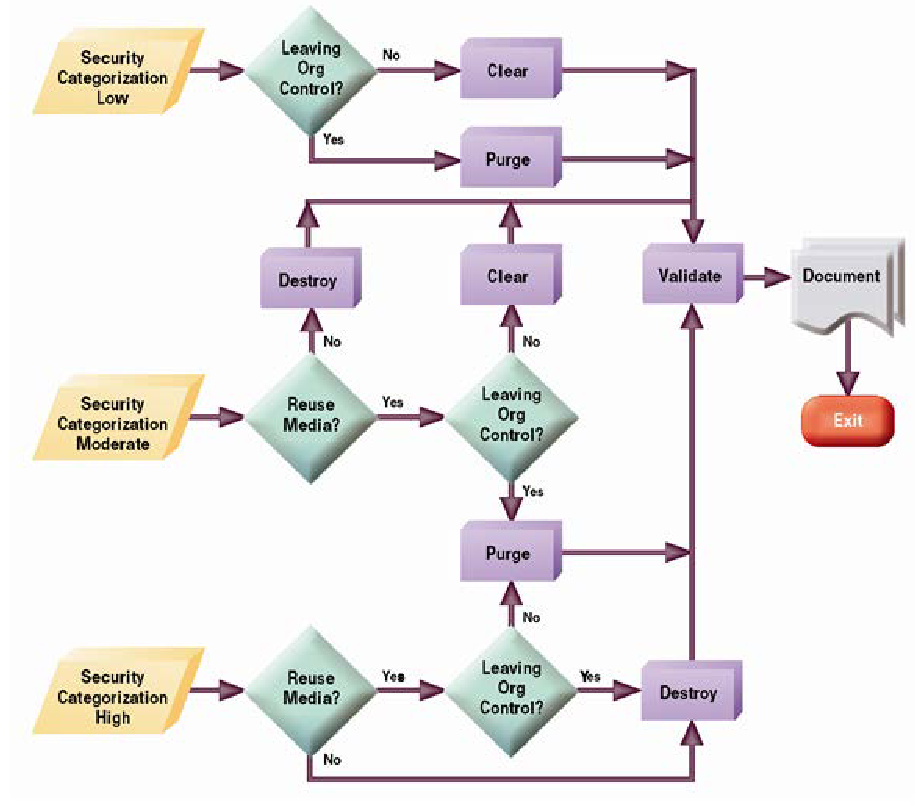
\includegraphics[height=2in]{screen1.png}
\end{frame}


\begin{frame}{Neo4J Property Graphs}

\begin{block}{Nodes}
\begin{itemize}
  \item May be labelled with zero, one or more labels
  \item Labels group nodes into sets
  \item Can have key--value pairs (''properties'')
\end{itemize}
\end{block}

\begin{block}{Relationships}
\begin{itemize}
  \item Directed, named connection between two nodes
  \item Typed with one relationship type
  \item Can have key--value pairs (''properties'')
  \item Can be navigated in any direction
\end{itemize}
\end{block}

\begin{block}{Path}
\begin{itemize}
  \item Sequence of alternating nodes and relationships
  \item Starts and ends at a node
\end{itemize}
\end{block}
\end{frame}

\begin{frame}{The Cypher Language}

\begin{block}{Basic Ideas}
\begin{itemize}
  \item Declarative (styled after SQL)
  \item Pattern matching (styled after SPARQL)
  \item Cypher query has multiple clauses (''query pipelines'')
  \item Read and write in a single Cypher statement
  \item Queries must return data
\end{itemize}
\end{block}
\end{frame}

\begin{frame}[fragile]{Cyper and Graph Concepts}
\centering
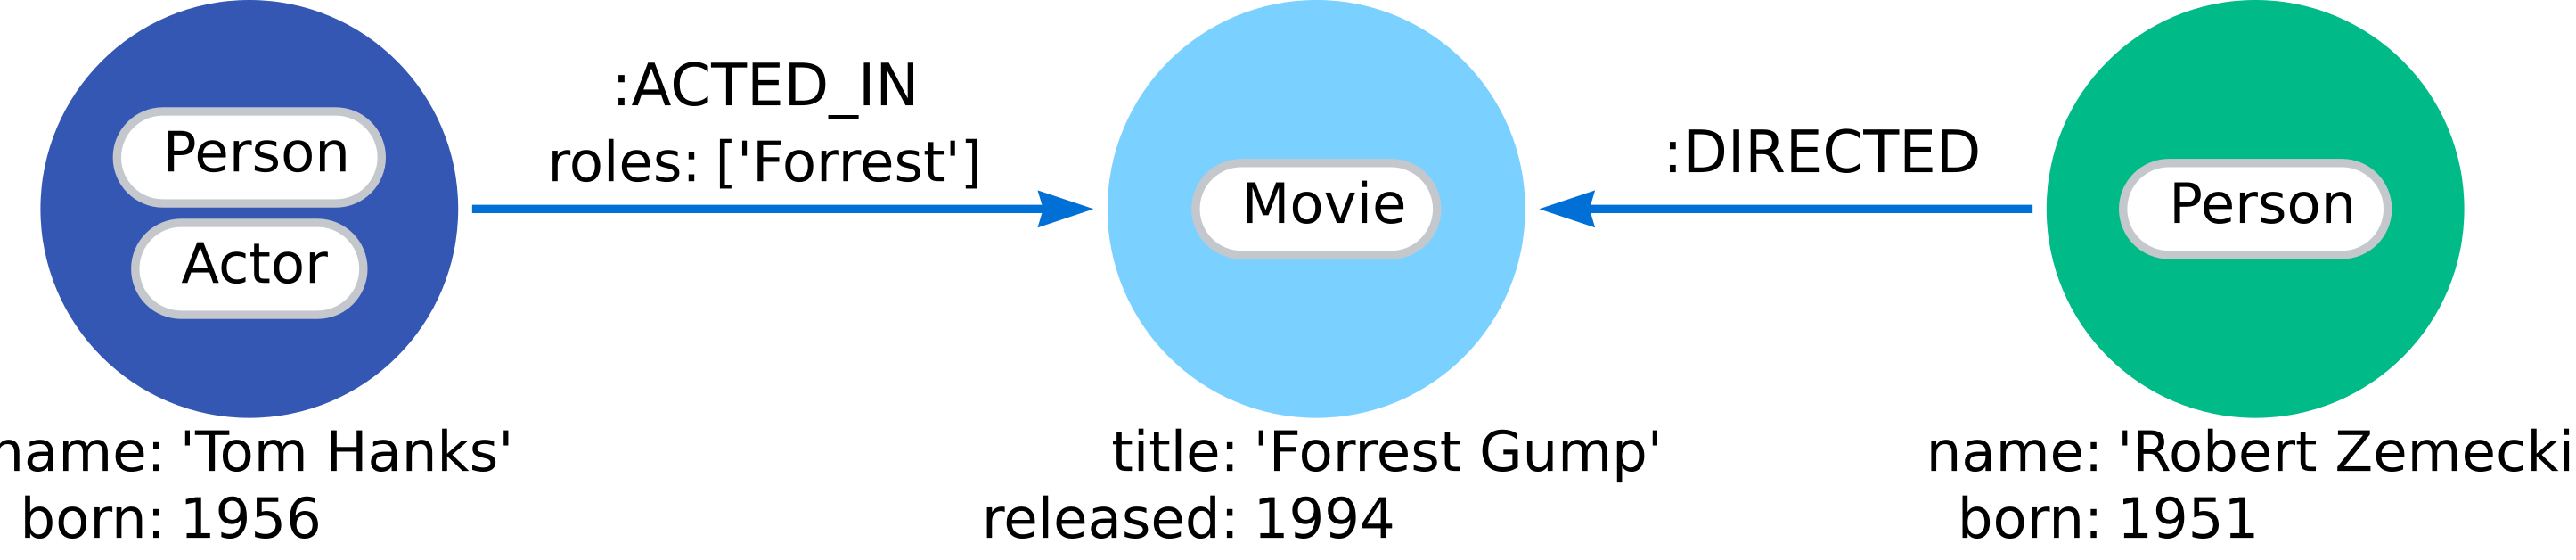
\includegraphics[width=\textwidth]{graph_simple-arr.png}
\tiny{\url{https://neo4j.com/docs/getting-started/_images/graph_simple-arr.svg}} \\
\vspace{\baselineskip}

\begin{cyphercode}
CREATE (:Person:Actor)
         -[:ACTED_IN {roles: ['Forrest']}]->
       (:Movie {title: 'Forrest Gump', released: 1994})
         <-[:DIRECTED]-
       (:Person {name: 'Robert Zemeckis', born: 1951})
\end{cyphercode}
\end{frame}

\begin{frame}{Cypher and Graph Concepts}
\centering
\includegraphics[width=\textwidth]{sample-cypher.png}
\tiny{\url{https://neo4j.com/docs/getting-started/_images/sample-cypher.svg}}
\end{frame}


\begin{frame}[fragile]{Cypher Syntax}
\begin{block}{Graph Nodes}
\centering

\textbf{\texttt{(variable : Label)}}

\begin{itemize}
  \item Optional variable name, optional label
\end{itemize}
\end{block}

\begin{block}{Relationships}
\centering

\textbf{\texttt{\;\;() - [variable : Label] - ()\;\;}} \\
\textbf{\texttt{\;\;() - [variable : Label] -> ()}} \\
\textbf{\texttt{() <- [variable : Label] - ()\;\;}} \\
\textbf{\texttt{\;\;() - - ()}\;\;} \\
\textbf{\texttt{() - ->()}}  \\
\textbf{\texttt{\;()<- - ()\;}} \\

\begin{itemize}
  \item Optional variable name, optional label
  \item Directionality matters for querying and must match that of the relationship as created
\end{itemize}
\end{block}

\end{frame}

\begin{frame}[fragile]{Cypher Syntax \small [cont'd]}
\small
\begin{block}{Node Properties}
\centering

\textbf{\texttt{(v:L \{ propertyName: propertyValue \} )}}
\end{block}

\begin{block}{Relationship Properties}
\centering

\textbf{\texttt{[r:L \{ propertyName: propertyValue \} ]}}
\end{block}

\begin{block}{Pattern}
\centering

\textbf{\texttt{(n1:L1 \{p1:v1\})-[r:L2 \{p2:v2\}]->(n2:L2 \{p3:v3 \})}}
\begin{itemize}
  \item Can be complex or simple
  \item Must be used with a keyword like MATCH for querying or like CREATE or MERGE for data definition
\end{itemize}
\end{block}
\end{frame}

\begin{frame}{Defining Graphs in Cypher}
\centering
\includegraphics[width=\textwidth]{screen4.png}
\tiny{\url{https://neo4j.com/docs/getting-started/_images/modeling_johnsally_properties-arr.svg}}
\end{frame}

\begin{frame}[fragile]{Defining Graphs in Cypher}

\scriptsize
\begin{cyphercode}
MERGE (j:Person {name: 'John'})
  ON CREATE SET j.age = 27
MERGE (s:Person {name: 'Sally'})
  ON CREATE SET s.age = 32
MERGE (b:Book {title: 'Graph Databases'})
  ON CREATE SET b.authors = ['Jim Webber', 'Ian Robinson']
MERGE (j)-[rel1:IS_FRIENDS_WITH]->(s)
  ON CREATE SET rel1.since = '01/09/2013'
MERGE (j)-[rel2:HAS_READ]->(b)
  ON CREATE SET rel2.on = '02/03/2013', rel2.rated = 5
MERGE (s)-[rel3:HAS_READ]->(b)
  ON CREATE SET rel3.on = '02/09/2013', rel3.rated = 4
\end{cyphercode}
\small
MERGE ensures a node or relationship exists in the graph, creating it if necessary; CREATE creates a node or relationship
%\vspace{3mm}
\scriptsize
\begin{cyphercode}
MATCH (n) RETURN n
\end{cyphercode}
\small
MATCH searches the graph for a pattern
\end{frame}

\begin{frame}{Defining Graphs in Cypher}
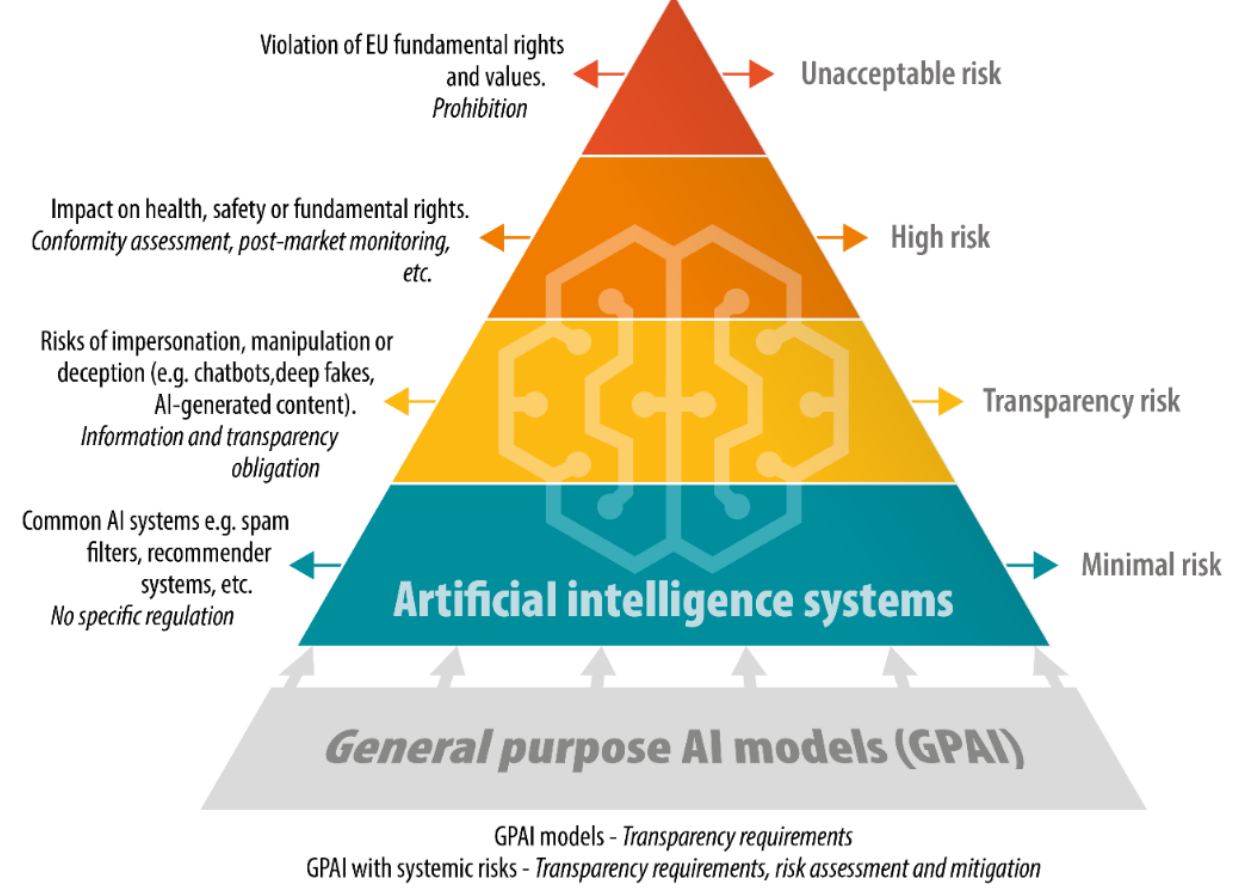
\includegraphics[width=\textwidth]{screen2.png}
\end{frame}

\begin{frame}{Hands-On Exercises}

Define a graph in Cypher that represents the following statement:\\

\begin{quote}
You are completing the course BUSI 4720 in this semester with a final grade of 100. BUSI 4720 is part of the BCom program where it is offered in the 4th year. BUSI 4720 carries 3 credit hours of academic credit. It is a course on the topic of Business Analytics. 
\end{quote}

\begin{enumerate}
  \item Identify nodes, relationships, and properties of nodes and relationships
  \item Use CREATE or MERGE statements to create nodes first, then relationships
  \item Use MATCH to verify your graph is correct.
\end{enumerate}
\end{frame}

\begin{frame}[fragile]{Clean-Up}
To remove Persons and Books and relationships between them:
\footnotesize
\begin{cyphercode}
MATCH (:Person|Book)-[r]-(:Person|Book) DELETE r;
MATCH (n:Person|Book) DELETE n;
\end{cyphercode}
\normalsize
Similar for other types of relationships or labels. \\

To remove \textbf{all} relationships and nodes use:
\footnotesize
\begin{cyphercode}
MATCH ()-[relationship]-() DELETE relationship;
MATCH (node) DELETE node;
\end{cyphercode}
\normalsize
\end{frame}

\begin{frame}[fragile]{Property or Relationship?}
\begin{columns}
\begin{column}{.35\textwidth}
\includegraphics[width=\columnwidth]{screen5.png}
\end{column}
\begin{column}{.65\textwidth}
\scriptsize
\begin{cyphercode}
//find the genres for 
// a particular movie
MATCH (m:Movie {title:"The Matrix"})
RETURN m.genre;

//find which movies share genres
MATCH (m1:Movie), (m2:Movie)
WHERE any(x IN m1.genre 
          WHERE x IN m2.genre)
AND m1 <> m2
RETURN m1, m2;
\end{cyphercode}
\end{column}
\end{columns}
\tiny{\url{https://neo4j.com/docs/getting-started/\_images/modeling\_genre\_property-arr.svg}}
\end{frame}

\begin{frame}[fragile]{Property or Relationship?}
\begin{columns}
\begin{column}{.35\textwidth}
\includegraphics[width=\columnwidth]{screen6.png}
\end{column}
\begin{column}{.65\textwidth}
\scriptsize
\begin{cyphercode}
//find the genres for a 
//particular movie
MATCH (m:Movie {title:"The Matrix"}),
      (m)-[:IN_GENRE]->(g:Genre)
RETURN g.name;

//find which movies share genres
MATCH (m1:Movie)-[:IN_GENRE]->(g:Genre),
      (m2:Movie)-[:IN_GENRE]->(g)
RETURN m1, m2, g
\end{cyphercode}
\end{column}
\end{columns}
\tiny{\url{https://neo4j.com/docs/getting-started/\_images/modeling\_genre\_node-arr.svg}}
\end{frame}

\begin{frame}{Flexible Data Modeling}
\centering
\includegraphics[height=1in]{screen7.png}
\tiny{\url{https://neo4j.com/docs/getting-started/_images/modeling_airport_flights-arr.svg}} \hrule
\includegraphics[height=2in]{screen8.png}
\tiny{\url{https://neo4j.com/docs/getting-started/_images/modeling_airport_flight_dates-arr.svg}}
\end{frame}

\begin{frame}{Graph Data versus Relational Data}
\centering
\includegraphics[height=1.2in]{screen9.png}
\tiny{\url{https://neo4j.com/docs/getting-started/_images/relational_model.svg}} \hrule
\includegraphics[height=1.8in]{screen10.png}
\tiny{\url{https://neo4j.com/docs/getting-started/_images/relational_graph_model-arr.svg}}
\end{frame}

\begin{frame}{Graph Data versus Relational Data}
\begin{block}{Conversion}
\begin{itemize}
  \item Tables to Node Labels
  \item Rows to Nodes
  \item Columns to Node Properties
  \item Foreign keys to Relationships
  \item Join tables to Relationships
  \item Remove NULL and default values
\end{itemize}
\end{block}
\end{frame}

\begin{frame}[fragile]{The Pagila Database for Neo4J}
Import the Pagila Datase (This may take ten or more minutes; already done in the course Virtual Machine):
\scriptsize
\begin{cyphercode}
CALL apoc.cypher.runFile(
'https://evermann.ca/busi4720/neo4j/import_pagila_from_csv.cypher')
\end{cyphercode}
\normalsize
Verify some data
\small
\begin{cyphercode}
MATCH (n:Actor) RETURN n LIMIT 25
\end{cyphercode}
\end{frame}

\begin{frame}{Explore the Pagila Graph}
\centering

\includegraphics[height=3in]{screen12.png}
\end{frame}

\begin{frame}[fragile]{Explore the Pagila Schema}
\small
\begin{cyphercode}
CALL db.schema.visualization()
\end{cyphercode}
\centering

\includegraphics[height=2.5in]{screen13.png}
\end{frame}

\begin{frame}[fragile]{Cypher Query Examples}
Find actors by last name, limit to 10
\footnotesize
\begin{cyphercode}
MATCH (a:Actor) 
RETURN a.firstName, a.lastName
ORDER BY a.lastName DESC
LIMIT 10;
\end{cyphercode}
\normalsize
Find films whose title starts with a 'T' and that have a rental rate less than 3, sort by film title, limit to 10
\footnotesize
\begin{cyphercode}
MATCH (f:Film {rating: 'PG'})
WHERE (f.title STARTS WITH 'T') AND (f.rentalRate < 3)
RETURN f.title, f.rating, f.rentalRate
ORDER BY f.title ASC LIMIT 10;
\end{cyphercode}
\end{frame}

\begin{frame}[fragile]{Cypher Query Examples \small [cont'd]}
Find rental customers that live in India
\footnotesize
\begin{cyphercode}
MATCH (r:Rental) 
        - [:RENTAL_CUSTOMER] -> (c) 
        - [:CUSTOMER_ADDRESS] -> () 
        - [:ADDRESS_CITY] -> ()
        - [:COUNTRY_OF_CITY] -> (ct {country: 'India'})
RETURN c.firstName, c.lastName, r.rentalDate LIMIT 5
\end{cyphercode}
\end{frame}

\begin{frame}{Hands-On Exercise}
\large
Find all customers that have rented a film with rating ''PG''\\
\normalsize
\begin{enumerate}
  \item Explore the graph visually in Neo4J browser, note the relationship types
  \item Consider the path from customer to film via rental and inventory
  \item Design a pattern that starts with a customer node and ends with a film node
  \item Define an appropriate WHERE clause of property restrictions in node patterns
\end{enumerate}
\end{frame}

\begin{frame}{Hands-On Exercise}
\includegraphics[width=\textwidth]{screen14.png}
\end{frame}


\begin{frame}[fragile]{Cypher Query Examples \small [cont'd]}
\textbf{Aggregation}: Find the mean and standard deviation of rental payments by country
\footnotesize
\begin{cyphercode}
MATCH (p:Payment) 
        - [:PAYMENT_RENTAL] -> (r:Rental) 
        - [:RENTAL_CUSTOMER] -> (c) 
        - [:CUSTOMER_ADDRESS] -> () 
        - [:ADDRESS_CITY] -> ()
        - [:COUNTRY_OF_CITY] -> (ct)
WITH ct, 
     avg(p.amount) AS amountMean, 
     stDev(p.amount) AS amountSD
RETURN ct.country, amountMean, amountSD
ORDER BY amountMean DESC LIMIT 5
\end{cyphercode}

\scriptsize
\url{https://neo4j.com/docs/cypher-manual/current/functions/aggregating/}
\end{frame}

\begin{frame}[fragile]{Cypher Query Examples \small [cont'd]}
\textbf{Collection}: Find the sets of last names of the movie cast, and the total number of actors
\footnotesize
\begin{cyphercode}
MATCH (a:Actor) - [:ACTS_IN] -> (f:Film) 
RETURN f.title, 
       collect(a.lastName) AS cast, 
       count(*) AS numActors;
\end{cyphercode}
\normalsize
\textbf{Collection}: Find the set ofs of film title by rental customer and the number of rentals
\footnotesize
\begin{cyphercode}
MATCH (f:Film) - [:FILM_INVENTORY] 
    - () - [:RENTAL_INVENTORY] 
    - (r:Rental) - [:RENTAL_CUSTOMER] 
    -> (c:Customer)
RETURN c.lastName, 
       collect(f.title) AS filmRentals, 
       count(*) AS numRentals;
\end{cyphercode}

\scriptsize
\url{https://neo4j.com/docs/getting-started/cypher-intro/results/}
\end{frame}


\begin{frame}[fragile]{Cypher Query Examples \small [cont'd]}
\textbf{Collection}: Find the set of rental customers for each film and the rental count
\footnotesize
\begin{cyphercode}
MATCH (f:Film) - [:FILM_INVENTORY] 
    - () - [:RENTAL_INVENTORY] 
    - (r:Rental) - [:RENTAL_CUSTOMER] 
    -> (c:Customer)
RETURN DISTINCT f.title, 
      collect(c.lastName+' '+left(c.firstName,1)+'.') 
          AS custNames, 
      count(*) as rentalCount
\end{cyphercode}
\end{frame}

\begin{frame}[fragile]{Cypher Query Examples \small [cont'd]}
\textbf{Sub-Query}: Find the customers who rent films that are in inventory at multiple stores
\footnotesize
\begin{cyphercode}
MATCH (c:Customer)<-[:RENTAL_CUSTOMER]
     -(r:Rental)-[:RENTAL_INVENTORY]
     -()-[:FILM_INVENTORY]
     -(f:Film) 
WITH c, count{ 
  MATCH (f)-[:FILM_INVENTORY]
       -()-[:STORE_INVENTORY]
       -(s:Store) 
  RETURN DISTINCT s.storeID
} AS storeNum
where storeNum > 1
RETURN DISTINCT 
  c.lastName
       +' '
       +left(c.firstName,1)
       +'.' AS custName, 
  storeNum
\end{cyphercode}
\end{frame}

\begin{frame}[fragile]{Cypher Query Examples \small [cont'd]}
Christian Akroyd's co-actors
\footnotesize
\begin{cyphercode}
MATCH (a:Actor {firstName: 'CHRISTIAN', 
                lastName: 'AKROYD'}) 
      - [:ACTS_IN] 
      - (f:Film) 
     <- [:ACTS_IN] 
      - (coActors) 
RETURN coActors.firstName + ' ' + 
       coActors.lastName AS Name;
\end{cyphercode}
\normalsize
\textbf{Quantified Relationships}: Movies and actors up to 2 ''hops'' away from Christian Akroyd
\footnotesize
\begin{cyphercode}
MATCH (a:Actor {firstName: 'CHRISTIAN', 
                lastName: 'AKROYD'})
      - [:ACTS_IN*1..2] 
      - (others) 
RETURN distinct others;
\end{cyphercode}
\end{frame}

\begin{frame}[fragile]{Cypher Query Examples \small [cont'd]}
\textbf{Built-In Function}: The shortest path of an acts-in relationship between Christian Akroyd and Charlize Dench
\footnotesize
\begin{cyphercode}
MATCH path=shortestPath( 
  (a1: Actor {firstName: 'CHRISTIAN', 
              lastName: 'AKROYD'}) 
  - [:ACTS_IN*] 
  - (a2: Actor {firstName: 'CHARLIZE', 
                lastName: 'DENCH'})) 
RETURN path;
\end{cyphercode}
\end{frame}

\begin{frame}[fragile]{Cypher Query Examples \small [cont'd]}
\textbf{Pattern in WHERE clause, multiple MATCH patterns} Find actors that Christian Akroyd hasn't yet worked with, but his co-actors have. Extend Christian Akroyd's co-actors, to find co-co-actors who haven't worked with him.
\footnotesize
\begin{cyphercode}
MATCH (a1:Actor {firstName:'CHRISTIAN', 
                 lastName:'AKROYD'})
      - [:ACTS_IN] -> (m) <-[:ACTS_IN] -(coActors),
  (coActors)-[:ACTS_IN]->(m2)<-[:ACTS_IN]-(cocoActors)
WHERE NOT (a1)-[:ACTS_IN]->()<-[:ACTS_IN]-(cocoActors) 
      AND a1 <> cocoActors
RETURN cocoActors.firstName+' '+
       cocoActors.lastName AS Recommended, 
       count(*) AS Strength 
ORDER BY Strength DESC
\end{cyphercode}
\end{frame}

\begin{frame}[fragile]{Cypher Query Examples \small [cont'd]}
Find someone who can introduce Christian Akroyd to Susan Davis
\footnotesize
\begin{cyphercode}
MATCH (a1:Actor {firstName:'CHRISTIAN', 
                 lastName:'AKROYD'})
          -[:ACTS_IN]->(m)<-[:ACTS_IN]-(coActors),
      (coActors)-[:ACTS_IN]->(m2)
      <-[:ACTS_IN]-(a2:Actor {firstName:'SUSAN', 
                              lastName:'DAVIS'})
RETURN a1, m, coActors, m2, a2
\end{cyphercode}
\end{frame}


\begin{frame}{Further Information}
\renewcommand{\arraystretch}{1.5}
\footnotesize
\begin{tabularx}{\linewidth}{l|X} \hline
Getting Started & \url{https://neo4j.com/docs/getting-started/} \\ 
Cypher Manual & \url{https://neo4j.com/docs/cypher-manual} \\
Graph Data Science & \url{https://neo4j.com/docs/graph-data-science} \\ 
APOC Library & \url{https://neo4j.com/docs/apoc/current/} \\ 
Use Cases & \url{https://neo4j.com/use-cases/} \\
Resources & \url{https://neo4j.com/resources/} \\
\hline
\end{tabularx}
\end{frame}

\begin{frame}{Hands-On Exercises}
\begin{enumerate}
	\item Are there two customers that have the same address?
	\item Which customers have rented the same set of films?
	\item Find all films with a single actor
	\item Calculate the rental revenue per customer. Who are the top 5? Bottom 5?
	\item Calculate the rental counts for each country of customer. Are there countries with no rentals?
	\item Create a graph that represents a product hierarchy.
\end{enumerate}
\end{frame}

\end{document}
